\documentclass[12pt,a4paper]{article} 
\usepackage[portuguese]{babel}
\usepackage[utf8]{inputenc}
\usepackage{adjustbox}
\usepackage{amsmath} 
\usepackage{graphicx}
\usepackage{booktabs}
\usepackage{float}
\begin{document}
\setcounter{figure}{4}
\setcounter{section}{3}
\setcounter{page}{5}
\section{Relatório}
\subsection{Introdução}

Nesta prática, deseja-se entender o funcionamento de um circuito integrado com um amplificador operacional, assim como analisar as características deste no domínio da frequência. Um amplificador operacional, ou amp-op, é um amplificador com ganho muito alto, uma impedância de entrada alta e uma baixa impedância de saída. Tipicamente, os usos típicos para amplificadores operacionais são para mudanças na amplitude de tensões (amplitude e polaridade), construção de osciladores, construção de filtros e muitos tipos de circuitos de instrumentação. Um op-amp contém vários estágios de amplificadores por diferença para que atinja um ganho de tensão, em malha aberta, muito alto. 

\subsection{Análises}
Do experimento 1 e 2, montaram-se as Tabelas de 1 a 4.

Do experimento 3, pode-se observar os seguintes gráficos com a ajuda de um osciloscópio:
\begin{figure}[htpb]
  \centering
  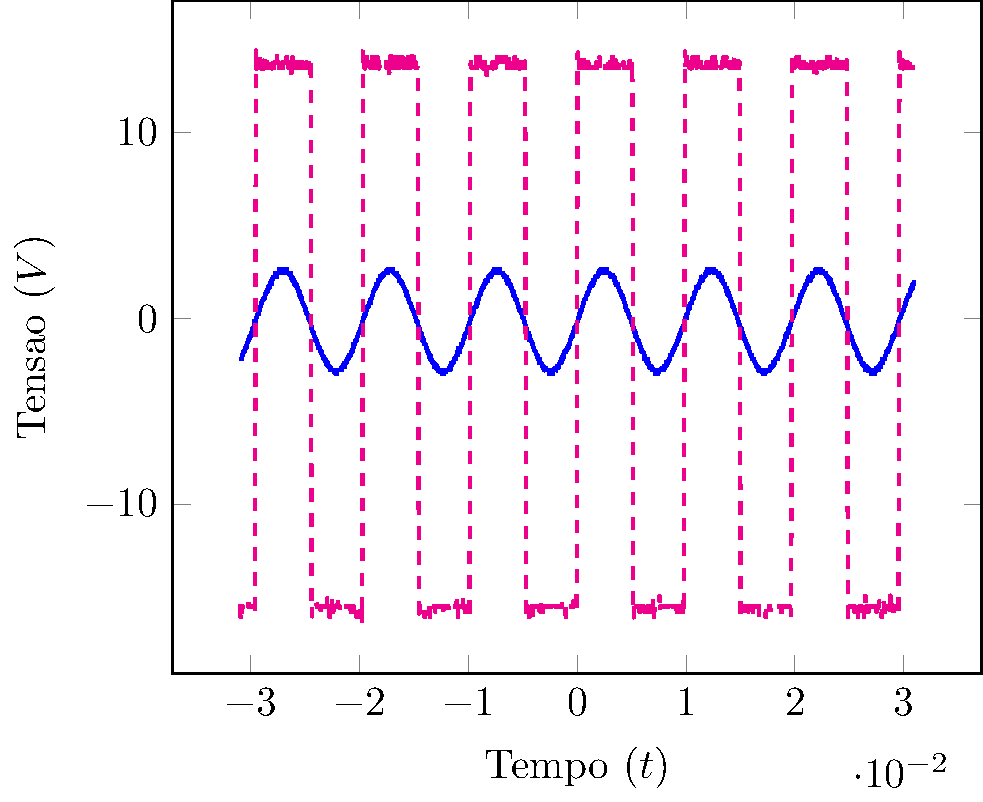
\includegraphics[width=0.8\linewidth]{./img/5V_100.pdf}
  \label{5V100}
\end{figure}

\begin{figure}[htpb]
  \centering
  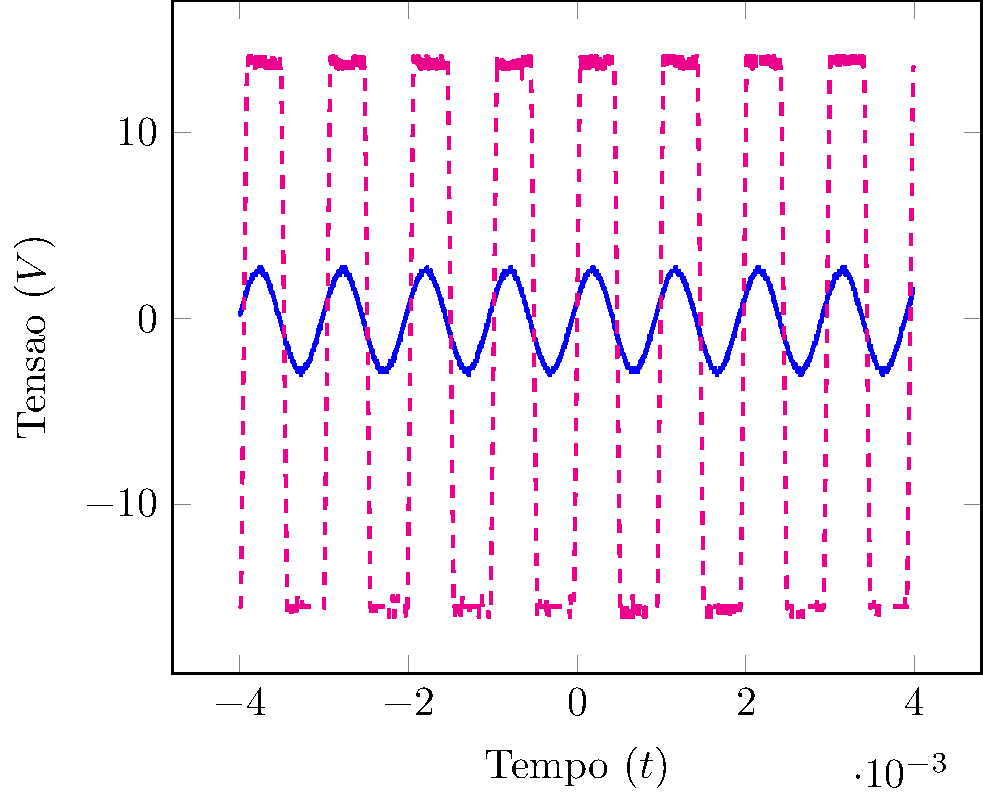
\includegraphics[width=0.8\linewidth]{./img/5V_1K.pdf}
  \label{5V1K}
\end{figure}
\begin{figure}[htpb]
  \centering
  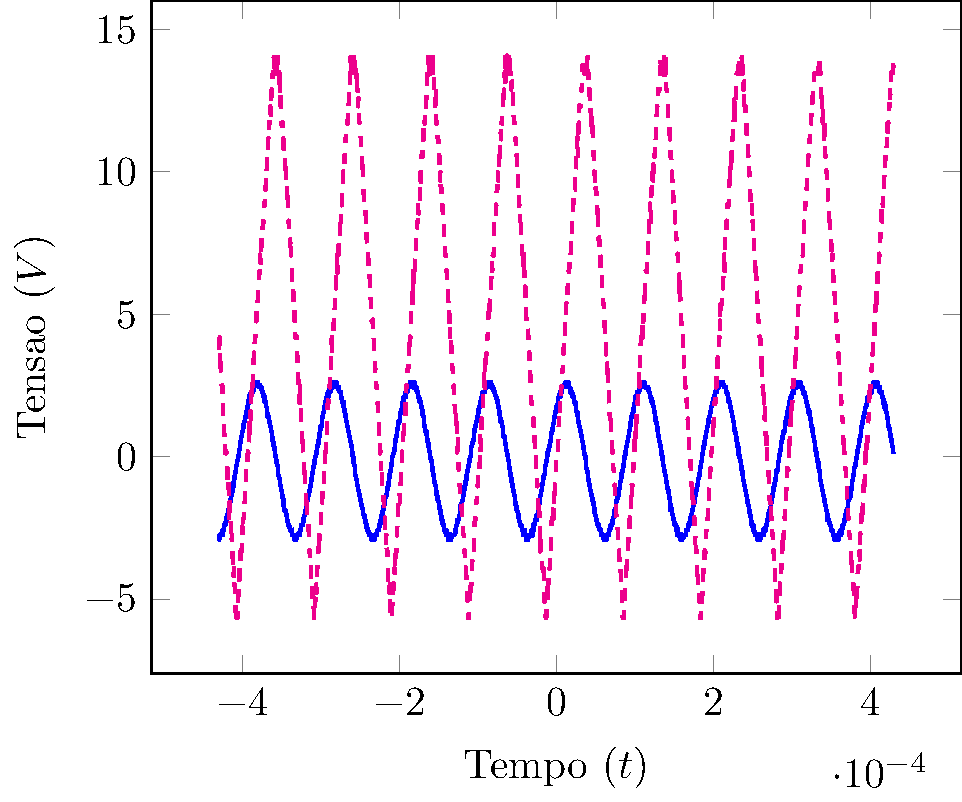
\includegraphics[width=0.8\linewidth]{./img/5V_100K.pdf}
  \label{5V100k.pdf}
\end{figure}
\begin{figure}[htpb]
  \centering
  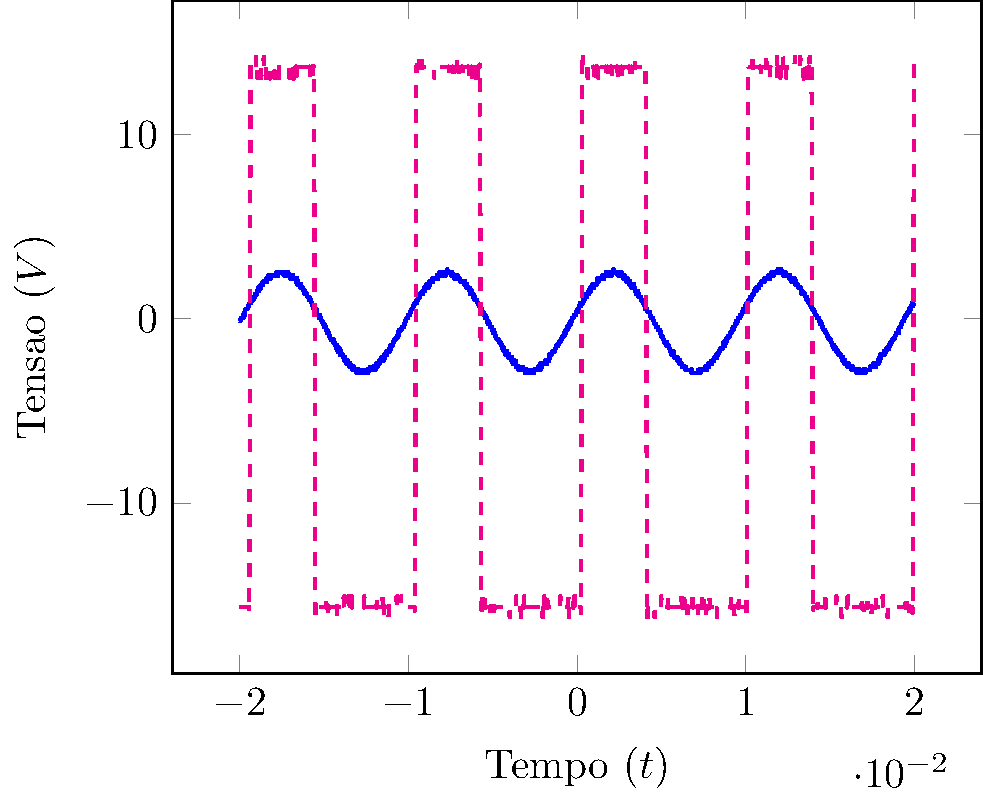
\includegraphics[width=0.8\linewidth]{./img/1V_100.pdf}
  \label{1V100}
\end{figure}
\begin{figure}[htpb]
  \centering
  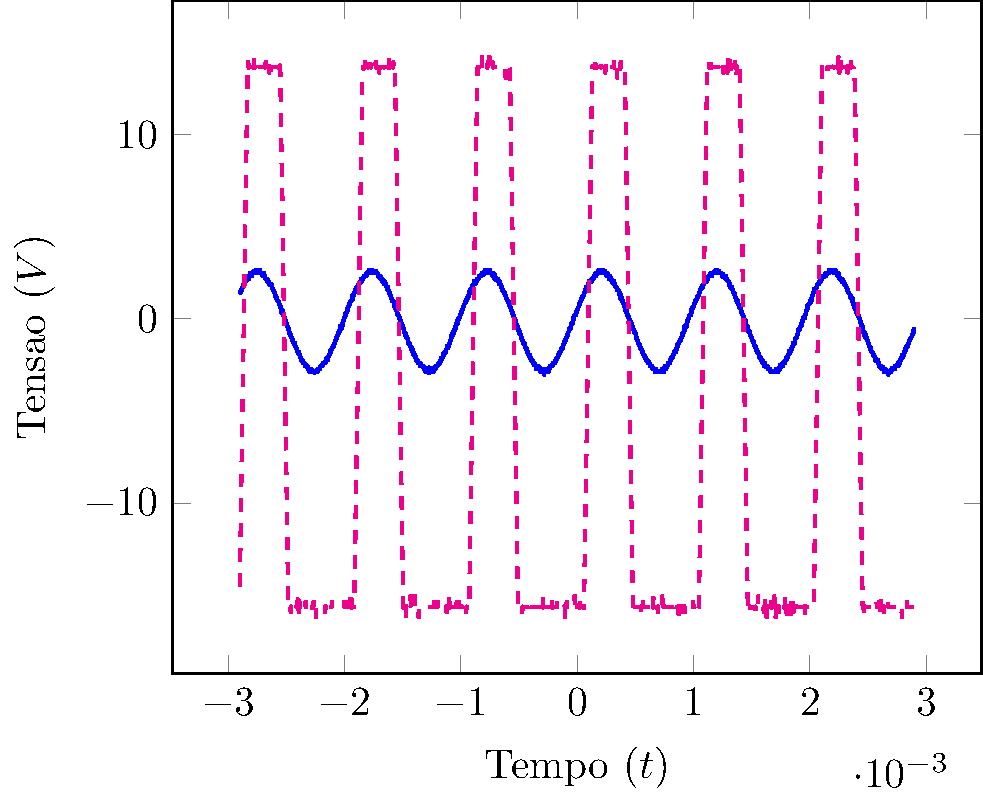
\includegraphics[width=0.8\linewidth]{./img/1V_1K.pdf}
  \label{1V1K}
\end{figure}
\begin{figure}[htpb]
  \centering
  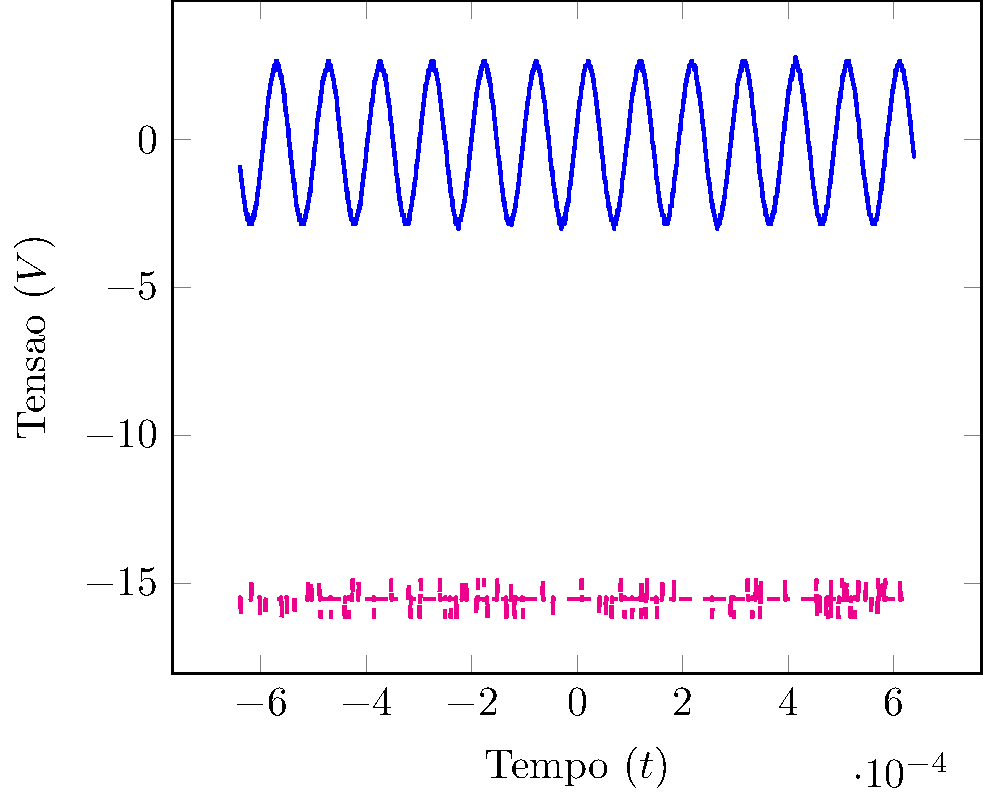
\includegraphics[width=0.8\linewidth]{./img/1V_100K.pdf}
  \label{1V100K}
\end{figure}
\begin{figure}[htpb]
  \centering
  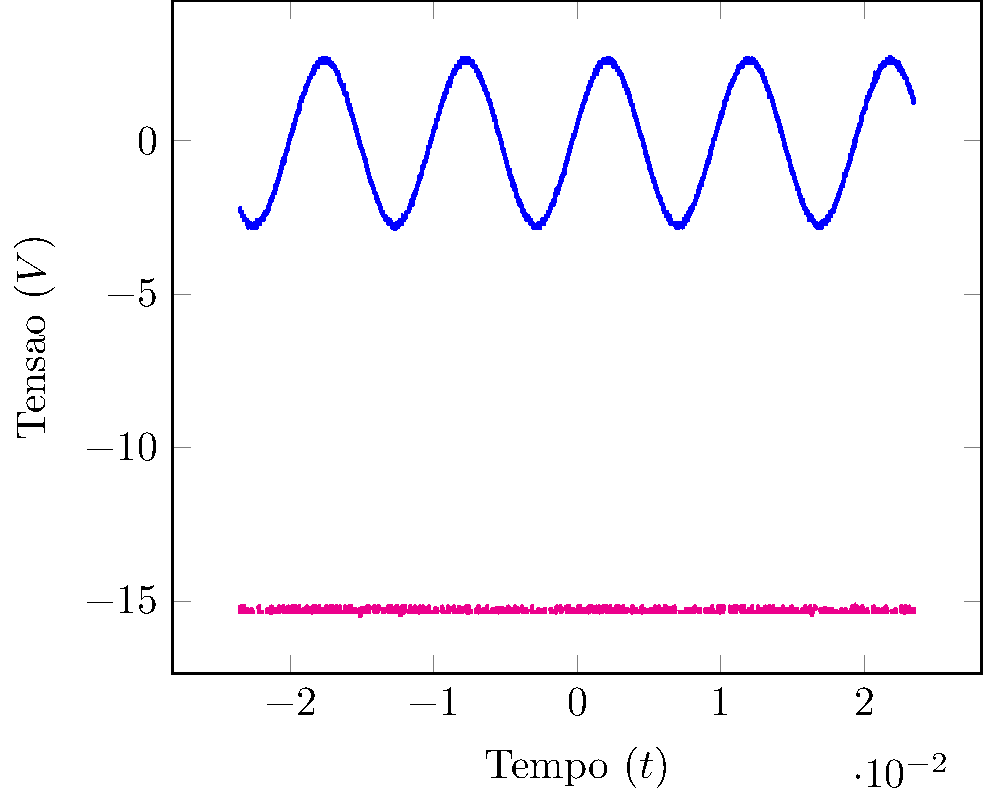
\includegraphics[width=0.8\linewidth]{./img/4V_100.pdf}
  \label{4V100}
\end{figure}
\begin{figure}[htpb]
  \centering
  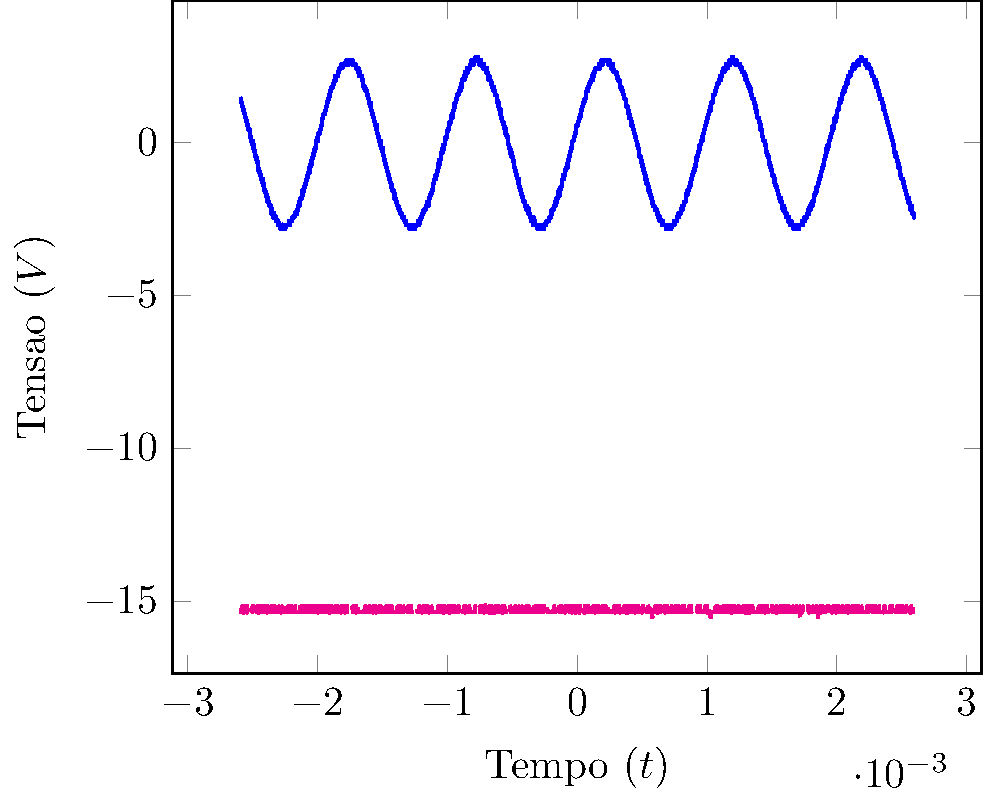
\includegraphics[width=0.8\linewidth]{./img/4V_1K.pdf}
  \label{4V1K}
\end{figure}
\begin{figure}[htpb]
  \centering
  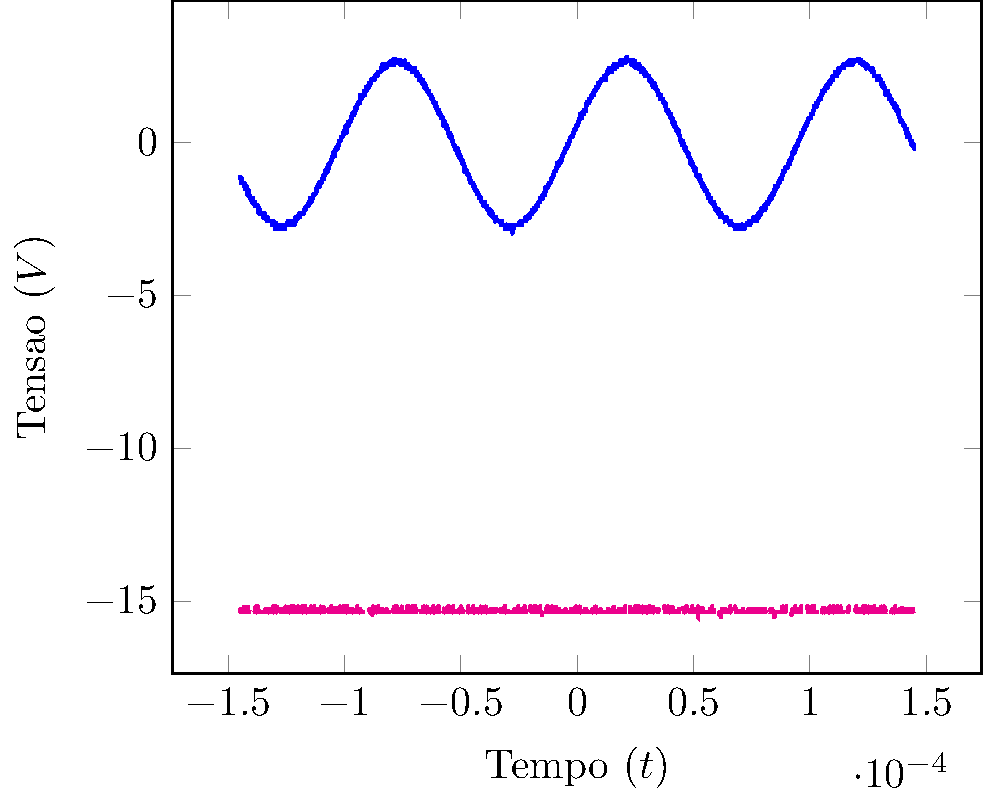
\includegraphics[width=0.8\linewidth]{./img/4V_100K.pdf}
  \label{4V100K}
\end{figure}
\subsection{Discussões}
O circuit inversor tem seu comportamento descrito pela Equação \ref{eq:1}. Desta forma, se temos um resistor $R_f =47 k\Omega$ e $R_1 = 4.7 k\Omega$, obteremos um ganho teórico de 10.
\begin{align}
  \label{eq:1}
G= - \frac{R_f}{R_1} 
\end{align}

Podemos assim, consultar a Tabela 1 e perceber que o ganho teórico se mantém na prática até a faixa dos $100 kHz$ para $1V$ e $10 kHz$ para $5V$. A partir destas frequências os ganhos dos amplificadores começam a descer de forma que a Equação \ref{eq:1} não prevê. Também observamos que, com uma entrada de $5V$ temos uma saturação na saída, pois alimentamos o amplificador com $-15V$ e $15V$, assim ele não consegue suprir tensões mais altas que $30V$.

A equação do amplificador não inversor é mostrado pela Equação \ref{eq:2}. O ganho teórico para o amplificador não inversor com $R_f = 47 k\Omega$ e $R_1=4.7 k\Omega$ seria $11V$. O que se 
\begin{align}
  G = 1 + \frac{R_f}{R_1} 
\end{align}
\subsection{Conclusão}
\end{document}
